\chapter{Symmetry-preserving basis optimization}
The splining techiniques presented in the last chapter open the door for optimizing the basis function without any additional cost at evaluation time (e.g. when running molecular dynamics).
We present in this chapter several optimization methods for the basis preserving symmetries that can be used in combination with splining that can be summarized by 
\begin{equation}
  \sum_{n}^{n_\textrm{max}}U_{qn}^{\lambda}(\mathcal{D}) c_{n\lambda} = c_{q\lambda}.
  %\sum_{an}\sum_m U_{xqan}^{\lambda} c_{anlm} = c_{xqlm}
  %\sum_n U_{qn}^{l} c_{anlm} = c_{nqlm} 5
  %\sum_n U_{qn}^{al}\langle anlm | \rho_i\rangle  = \langle aqlm | \rho_i\rangle
\end{equation}
The linear transformation $\mathbf{U}$ computed from dataset $\mathcal{D}$ recombines the radial expansion coefficients for a fixed basis $\{b_{n}^\lambda\}_{n=1}^M$ resulting in optimized coefficients $c_{q\lambda}$.
The idea is that the initial basis is chosen to cover a large hypothesis space $\mathcal{H}$, the optimized basis is optimal wrt. to a dataset $\mathcal{D}\subset\mathcal{H}$.
The optimized coefficients can be then truncated at $M^\prime$ with the hope that $M^\prime << M$.
Such that the featurization is much lower dimensional space reducing the number of computational steps when predicting a property.
Constraining $\mathbf{U}$ to be linear allows the use of the splining as the targeted function is not changed
%basis function changes its dimensionality
\begin{equation}
  \sum_n U_{qn}^{\lambda} c_{n\lambda} R_{n\lambda}(r) = c_{q\lambda} R_{q\lambda}(r)
\end{equation}
Then the splining as described in Eq.~\ref{TODO} is constructed for the radial coefficients $c_{q\lambda}$ such that the transformation $\mathbf{U}$ can be bypassed during evaluation.
\begin{figure}
    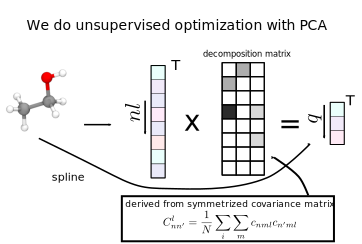
\includegraphics[width=\textwidth]{fig/slide22_0.png}
    \caption{A schematic showing the spline trick. TODO use poster spline trick as basis maybe add more description about the optimization.}
    \label{fig:spline_trick}
\end{figure}

TODO do we need orthogonality?

%\label{sec:evaluation_of_radial_contribution}
%An efficient implementation for the evaluation of the radial basis function in the spherical expansion for the computation of SOAP was part of my work in the first year.
%Therefore the recent developments of efficient schemes are here discussed in more detail.
%Following the Eq.~\ref{eq:soap} for the SOAP descriptor by resolving the expansion on the angular contribution results in
%\begin{equation}
%\label{eq:radial_part_in_spherical_expansion}
%%\langle rlm|\mathcal{X}_i\rangle =  4\pi\underbrace{\exp[-a(r^2+r_{ij}^2)]i_l(2ar_{ij})}_{\text{radial term}}Y_{l}^m(\alpha_{ij},\beta_{ij}),
%\langle rlm|\mathcal{X}_i\rangle_{\hat{R}} \propto \sum_{j\in\mathcal{X}_i}\exp[-a(r^2+r_{ij}^2)]i_l(2arr_{ij})Y_l^m(\hat{\mathbf{r}}_{ij}),
%\end{equation}
%where $i_l$ is the modified spherical Bessel function of the first kind.
%%and ($\theta{ij},\phi{ij}$ are the spherical coordinates of the unit vector $\hat{\mathbf{r}}$
%For an effective radial basis function, higher-order polynomials have been used in the first version of SOAP\cite{bartok2013representing}
%\begin{equation}
%R_n^{poly}(r) = (r_{\text{cut}} - r)^{n+2}N_n,\quad N_n\text{ is a normalization parameter.}
%\end{equation}
%The disadvantage is that the expansion has no analytic solution and is therefore performed with a least square fitting. %\cite{https://github.com/libAtoms/QUIP/issues/100#issuecomment-376115320}
%A proposed solution to this problem is to remove the dependency of the radial term on the spherical Bessel function by separating the angular and radial part in the atom density function\cite{caro2019optimizing}
%\begin{equation}
%g(\mathbf{r} - \mathbf{r}_j) \approx \tilde{g} = g_{r}(r)g_{\perp r}(\hat{\mathbf{r}},\mathbf{r}_j).
%\end{equation}
%The radial part can be then simplified to
%\begin{equation}
%\langle rlm|\mathcal{X}_i\rangle_{\hat{R},\tilde{g}} \propto \sum_{j\in\mathcal{X}_i} b(r_{ij})\exp[-a(r^2+r_{ij}^2)]Y_l^m(\hat{\mathbf{r}}_{ij}),
%\end{equation}
%% In the paper there is still a smooth cutoff function dependent on r, but this one is omitted here
%where $b(r_{ij})$ is a factor dependent only on $r_{ij}$.
%This allows an analytic expansion on higher-order polynomials.
%%For my work I followed a different approach as described in detail in the subsequent Section~\ref{sec:cubic_spline}.

\section{Closed-form solutions}
%The target of the optimization are the radial expansion coefficients in Eq.~\ref{eq:radial_expansion}
%\begin{equation}
%  c_{nl} = c_{n\lambda} c_{\lambda\mu}.
%\end{equation}
%
%\begin{equation}
%  \int\mathrm{d}\mathbf{r} \rho(\mathbf{r})\rho(\mathbf{r}^\prime)\,
%\end{equation}
%
%\begin{equation}
%  \sum_n U_{qn}^{al}\langle anlm | \rho_i\rangle  = \langle aqlm | \rho_i\rangle
%  %\langle anlm \lambda|\rho_i\rangle 
%  %\langle lm|\rho_i\rangle = <a^\prime n^\prime l|\rho_i> <lm|\rho_i>
%\end{equation}
We dicuss here optimizations that have closed-form solution for the computation of $U$.
Such solutions are typically faster to compute but also less accurate.

Closed-solution are usually more efficient in computation time, but often only improve the basis by linear transformation or fixed subset of nonlinear transformation.
\subsection{Unsupervised optimization}
Principal component analysis has been proposed to compute the data-driven contractions of equivariant features that represent in the most informative way the variability of a dataset as part of the N-body iterative contraction of equivariant (NICE) frameworks.~\cite{niga+20jcp}
We propose to apply this procedure on the first-order equivariants -- that correspond to the density coefficients -- as a mean to determine a data-driven radial basis. 
Keeping different chemical species separate, this amounts to computing the rotationally invariant covariance matrix (see SI) 
%In Ref.~\citenum{niga+20jcp} it has been proposed to use principal component analysis to compute the data-driven contractions of equivariant features that best represent the variability of a dataset.
%In combination with an iterative expression to compute density correlations of increasing order, this idea underlies the N-body iterative contraction of equivariant (NICE) frameworks. 
%The procedure can be readily applied to the first-order equivariants -- that are equal to the density coefficients. Keeping different chemical species separate, this amounts to computing the rotationally invariant covariance matrix (see SI)
\begin{equation}
C^{al}_{nn^\prime}= \frac{1}{N} \sum_i \sum_m <an l m|\rho_i> <\rho_i|an^\prime lm>,
\label{eq:cov}
\end{equation}
where the summation over $m$ ensures that the covariance is independent of the orientation of structures in the dataset.
For each $(a, l)$ channel, one diagonalizes $\mathbf{C}^{al}=\mathbf{U}^{al} \mathbf{Lam}^{al} (\mathbf{U}^{al})^T$, and computes the optimal coefficients
\begin{equation}
%<aq lm; opt||\rho_i> = \sum_n U^{al}_{qn} <an lm|\rho_i>. \label{eq:contract}
\end{equation}
Note that we compute $\mathbf{C}^{al}$ without centering the density coefficients. For $l>0$, the mean ought to be zero by symmetry (although it might not be for a finite dataset), and even for the totally symmetric, $l=0$ terms, density correlation features are usually computed in a way that is more consistent with the use of non-centered features. 

The number of contracted numerical coefficients $\qmax$ can be chosen inspecting the eigenvalues $\Lambda^{al}_q$.
At first, it might appear that in order to evaluate the contracted basis one has to compute the full set of $\nmax$ coefficients, and this is how the idea was applied in Ref.~\citenum{niga+20jcp}. 
When combining Eq.~\eqref{eq:contract} with Eq.~\eqref{eq:neighbor-sum}, however, one sees that the contracted coefficients can be evaluated directly 
\begin{equation}
\!\!\rep<aqlm; \opt||\rho_i> \!=\! \sum_j \delta_{\e\e_j} \rep<aql; \opt||r_{ji}; g>\! \rep<lm||\brhat_{ji}>,
\label{eq:neighbor-contract}
\end{equation}
using the contracted radial integrals
\begin{equation}
\rep<aq l; \opt||r; g> = \sum_n U^{al}_{qn} \rep<nl||r; g>, \label{eq:contract-integral}
\end{equation}
, and then evaluated at exactly the same cost as for a spline approximation of the radial integrals of a primitive basis of size $\qmax$.
Splining does not affect the equivariant behavior of the atom-density features, and introduces minute discrepancies relative to the analytical basis that do not affect the quality of the resulting models. 

%\subsubsection{Mixed-species basis}
Even though Eq.~\eqref{eq:cov} is defined separately for different species $a$, it is also possible to compute cross-correlations between different elemental channels, defining
\begin{equation}
 C^{l}_{an; \e'n'}= \frac{1}{N} \sum_i \sum_m \rep<an l m||\rho_i> \rep<\rho_i||\e' n' lm>,
\label{eq:cov-multispecies}
\end{equation}
as done in the NICE framework\cite{niga+20jcp} following ideas proposed in Ref.~\citenum{will+19jcp}, resulting in coefficients that combine information on multiple species
\begin{equation}
\rep<q lm; \opt||\rho_i> = \sum_n U^{l}_{q;an} \rep<an lm||\rho_i>, \label{eq:contract-multispecies}
\end{equation}
similar in spirit to the alchemical contraction discussed in Ref.~\citenum{will+18pccp}.
It is worth noting that although the NICE code\cite{NICE-REPO} contains the infrastructure to compute these contractions \emph{as a post-processing of the primitive basis}, the implementation we propose in  \texttt{LIBRASCAL} computes the contracted coefficients directly. However, it only implements the less information-efficient separate $(a, n)$-PCA strategy.
An implementation that evaluates directly the combined contraction would incur an overhead because every neighbor would contribute to every $q$ channel irrespective of their species:
\begin{multline}
%\rep<qlm; \opt||\rho_i>  = \sum_j \sum_{an} U^l_{q; an} \delta_{a\e_j}
%\rep<nlm||\br_{ji}; g>  \\
%= \sum_j \sum_{n} U^l_{q; \e_j n} \rep<nl||r_{ji}; g>\rep<lm||\brhat_{ji}> \\=
%\sum_j \rep<\e_j q l; \opt||r_{ji}; g>\rep<lm||\brhat_{ji}>.
\end{multline}
Given however that the cost of evaluating the density coefficients is usually a small part of the calculation of density-correlation features\cite{caro19prb,musi+21jcp}, we expect that this approach should be in general preferable compared to the calculation of a large primitive basis, and to a two-step procedure in which element-wise optimal functions are further contracted into mixed-element coefficients.

\subsubsection{Example: Collective variable optimization}
We can see that we can retrive similar quality CV as in the BaTiO3 paper from a snapshot.
Applying PCA is not a new thing, as it is a chicken-egg problem.

\subsection{Supervised optimization}
%\alexnote{I find this title confusing, since we never refer to supervised selection. For me something like "Beyond unsupervised decomposition" would make more sense, since this is what we introduced in the last paragraph.}
For a given number of radial functions, and a target data set, the data-driven contracted basis~\eqref{eq:contract} provides the most efficient description of the atom-centred density in terms of the fraction of the retained variance.
%The basis construction by the covariance matrix guarantees 
The most effective variance-preserving compression however does not guarantee that the features are the most effective to predict a given target property.
In fact, it has already been shown that SOAP features tend to emphasize correlations between atoms that are far from the atomic center, which can lead to a counter-intuitive degradation of the model accuracy with increasing cutoff radius\cite{bart+17sa,will+18pccp}. 
This effect can be contrasted by introducing a radial scaling\cite{huan-vonl16jcp,will+18pccp} that de-emphasizes the magnitude of the atom density in the region far from the central atom. 
By applying this scaling -- or other analogous tweaks\cite{caro19prb} -- to the atom density before it is expanded in the primitive basis, one ensures that the optimal basis is also built with a similar focus on the structural features that contribute more strongly to the target property.
In other terms, the information-optimal basis set we introduce here can be combined with a heuristic or data-driven optimization of the underlying density representation, to reflect the scale and resolution of the target property.

Another possibility is to extend the scheme to incorporate a supervised target $y_i$ in the selection of the optimal basis using principal covariates regression (PCovR) \cite{dejo-kier92cils,helf+20mlst}.
PCovR is a simple linear scheme that can be tuned to provide a projection of features to a low-dimensional latent space that combines an optimal variance compression target with that of providing an accurate linear approximation of the desired target property. 
Since $l>0$ contributions of the features have zero mean, the optimization problem can be combined with a supervised component only for $l=0$, and yields an optimal basis
\begin{equation}
<r||  aq 0; \opt; \gamma> = \sum_n U^{\e0;\gamma}_{qn} <r||n0>,
\end{equation}
which is a special case of Eq.~\eqref{eq:contract-basis} for $l=0$, 
where $U^{\e0;\gamma}_{qn}$ is obtained as the orthogonalized PCovR projector, as discussed in Refs.~\citenum{dejo-kier92cils,helf+20mlst}, using a mixing parameter $\gamma$, that determines how strong the emphasis of the optimization should be on minimizing the residual variance or the error in regressing the target.

\begin{multline}
<Q;\nlk||\frho[\gslm]_i^{(\nu+1)}>\propto 
\sum_{m}   <n||\frho[\lm]_i^1>\times\\[-1mm]
<Q||\frho[\sigma((-1)^{l+k+\lambda}); k (\mu-m)]_i^{\nu}>  \cg{\lm}{k (\mu-m)}{\glm},
\end{multline}
using Clebsch-Gordan coefficients $\cg{lm}{l'm'}{l''m''}$ in an expression analogous to the sum of angular momenta.
The $\nu=1$ equivariants are nothing but the density coefficients
\begin{equation}
<n||\frho[\sigma;\lm]_i^1>  = \delta_{\sigma 1}<\nlm||\rho_i>^\star,
\end{equation}
and one can compute invariant descriptors by retaining only the $<Q|\frho[1; 00]_i^\nu>$ terms, using the other components only as computational intermediates.

\section{Higher-order information}
Most NN structures use the approach to find a radial basis that is simple to evaluate to then let the NN optimize the basis.
Due to the flexible optimization space of NN, they can achive quite good accuracies which would not been able to achive with shallow methods\cite{schutt2018schnet}.
%In several architectures the time Dirac delta function is used, since the expansion coefficient is given by the distance.
\begin{figure}
    \includegraphics[width=\textwidth]{fig/slide23_0.png}
    \caption{Nonlinear the equivariant optimization by gradient descent}
    \label{fig:nonlinear-basis-opt}
\end{figure}

% guillaume/natashas work
\section{Future directions}
\subsection{Hierarchical optimization}
\papercomment{Optimizing first the chemical part and then the radial part, because optimizing both seems not to work well}\\
In the work of Natasha \& Guillaume the optimzation of radial and chemical due to the huge optimization space.
It is well known that deep NN have an equivalent functional form with one layer, but the learning peformance is dramatically better in the former one.
Both the radial and species channel increase the feature size by a multiplicative factor and thereby also the weigh matrix size.
%using low number of  %TODO find citation.
%Optimization in t case is tricky, since huge matrices multiplcation are not so closed-form optimizations
\subsection{Radial dependent smoothness}
\papercomment{make sigma dependent on r, because we see that it works well for GTOs}
% LE basis, radial smoothening
